\documentclass[runningheads,a4paper]{llncs}
\usepackage{amsmath,amssymb,booktabs,graphicx,microtype,url,xspace,float}
\usepackage[ruled,vlined,linesnumbered]{algorithm2e}
\usepackage{tikz}
\usepackage{marvosym}
\usetikzlibrary{arrows.meta,positioning,calc}
\newcommand{\vol}{\operatorname{vol}}
\newcommand{\HT}{H^{T}}
\newcommand{\NEST}{NEST\xspace}
\ifdefined\withappendix
  \newcommand{\proofdetails}{Appendix~\ref{app:proofs}}
  \newcommand{\ablationdetails}{Table~\ref{tab:ablation}}
\else
  \newcommand{\ablationdetails}{the supplementary appendix}
  \newcommand{\proofdetails}{the supplementary proof appendix}
\fi
\newcommand{\NESTGainVsHCSE}{0.5468}
\newcommand{\NESTGainVsHCSECI}{0.0218}
\newcommand{\NESTGainVsBBM}{0.5213}
\newcommand{\NESTGainVsBBMCI}{0.0101}
\newcommand{\NESTGainVsBestExternal}{0.4239}
\newcommand{\NESTGainVsBestExternalCI}{0.0086}
\newcommand{\OursWins}{500/500}
\newcommand{\OursWithinOne}{500/500}
\newcommand{\AuditOneRate}{69\%}
\newcommand{\AuditCompoundRate}{50\%}
\newcommand{\RealWins}{4/4}
\newcommand{\FairNESTExact}{249/250}
\newcommand{\FairHCSEExact}{2/250}
\newcommand{\FairBBMExact}{1/250}
\newcommand{\FairNESTMeanGap}{0.00032\%}
\newcommand{\FairNESTWorstGap}{0.07990\%}
\newcommand{\ScaleNFourteenExact}{99/100}
\newcommand{\ScaleNSixteenExact}{22/25}
\newcommand{\ScaleCombinedExact}{370/375}

% Generated by scripts/make_purity_macros.py; do not edit.
\newcommand{\PurityFineNEST}{0.546}
\newcommand{\PurityFineHCSE}{0.483}
\newcommand{\PurityFineGainHCSE}{0.062}
\newcommand{\PurityFineGainHCSECI}{0.005}
\newcommand{\PurityFineLowerHCSE}{61/500}
\newcommand{\PurityFineBBM}{0.486}
\newcommand{\PurityFineGainBBM}{0.060}
\newcommand{\PurityFineGainBBMCI}{0.007}
\newcommand{\PurityFineLowerBBM}{99/500}
\newcommand{\PurityCoarseNEST}{0.681}
\newcommand{\PurityCoarseHCSE}{0.601}
\newcommand{\PurityCoarseGainHCSE}{0.081}
\newcommand{\PurityCoarseGainHCSECI}{0.007}
\newcommand{\PurityCoarseLowerHCSE}{60/500}
\newcommand{\PurityCoarseBBM}{0.571}
\newcommand{\PurityCoarseGainBBM}{0.110}
\newcommand{\PurityCoarseGainBBMCI}{0.010}
\newcommand{\PurityCoarseLowerBBM}{76/500}

% Generated by scripts/make_review3_macros.py; do not edit.
\newcommand{\CertGraphs}{500/500}
\newcommand{\CertBinary}{500/500}
\newcommand{\CertFromAgg}{333}
\newcommand{\CertFromParis}{167}
\newcommand{\CertMaxDescent}{41}
\newcommand{\CertMaxCompound}{5}
\newcommand{\BBMBudgetHits}{71/500}
\newcommand{\MaxBarrier}{0.008}
\newcommand{\HCSEMaxDistinct}{3}
\newcommand{\BBMDistinctRange}{3--23}
\newcommand{\SensBSixtyFourGain}{0.0055}
\newcommand{\SensBSixtyFourLower}{31/50}
\newcommand{\SensBFourLoss}{0.0014}
\newcommand{\SensBFourHigher}{21/50}

\emergencystretch=2em
\raggedbottom
\widowpenalty=10000
\clubpenalty=10000
\displaywidowpenalty=10000
\setlength{\textfloatsep}{10pt plus 2pt minus 2pt}
\setlength{\floatsep}{8pt plus 2pt minus 2pt}
\setlength{\intextsep}{8pt plus 2pt minus 2pt}

\begin{document}
\title{NEST: Locally Certified Search for\\
Structural-Entropy Hierarchies}
\titlerunning{NEST: Certified Structural-Entropy Hierarchy Search}
% Affiliations as in the CIKM 2026 camera-ready; Yicheng Pan is the sole corresponding author.
\author{Dingli Su\inst{1}\and
Yicheng Pan\inst{1}\textsuperscript{(\Letter)}\and
Angsheng Li\inst{1,2}}
\authorrunning{D. Su et al.}
\institute{State Key Laboratory of Complex \& Critical Software Environment,
Beihang University, Beijing, China\\
\email{$\{$sudingli,yichengp,angsheng$\}$@buaa.edu.cn}\and
Zhongguancun Laboratory, Beijing, China}
\maketitle

\begin{abstract}
Structural entropy evaluates a graph hierarchy through the description length
of an encoding tree. HCSE and BBM \cite{pan2025} construct such trees but do not
determine whether the result admits a local entropy-reducing topology change.
We introduce NNI-certified Entropy Search over Trees (\NEST), a multi-start
optimizer based on rooted nearest-neighbor interchange (NNI). For weighted
graphs, we derive the exact NNI entropy change and prove that an improving
rotation can be inaccessible to a monotone merge or compression. The formula
supports best-improvement descent and a checkable one-NNI local-optimality
certificate. Because a better tree may require a temporary increase, \NEST also
tests bounded two-move paths but commits only improving endpoints. We also
formulate an $O(3^n)$ subset dynamic program, using binary sufficiency
\cite{zhang2021supertad,pan2025}, to compute exact global optima for audit
graphs. Across 500 graphs from five 64-vertex
hierarchical regimes, \NEST lowers entropy by
$\NESTGainVsBestExternal\!\pm\!\NESTGainVsBestExternalCI$ bits relative to the
better of HCSE and BBM and wins all 500 paired comparisons. In sealed,
candidate-budget-matched audits, 32 coalescent starts reach the exact global
optimum on 249/250, 99/100, and 22/25 instances at $n=12,14,16$, respectively
(\ScaleCombinedExact{} overall), whereas 32-call HCSE and label-free BBM reach
2/375 and 1/375. These finite audits measure observed optimality on the
declared suites; they do not establish an approximation ratio.
\keywords{Structural entropy \and hierarchical clustering \and tree editing
\and nearest-neighbor interchange \and graph algorithms}
\end{abstract}

\section{Introduction}
Many networks are organized at more than one scale: vertices form local
groups, related groups form larger modules, and the desired output is therefore
a tree rather than one flat partition. Structural entropy supplies an
information-theoretic objective for such an encoding tree \cite{li2016}.
Recent HCSE and BBM methods construct low-entropy hierarchies through recursive
partitioning and balanced merging \cite{pan2025}. Their construction rules
leave a complementary question unanswered: \emph{after construction, can a
local topology change further reduce structural entropy?}

A hierarchy constructor can make an early merge that later steps never revisit,
even when rotating a nearby internal edge would lower structural entropy. We
therefore seek a topology operator whose effect can be computed exactly, whose
termination certifies the inspected neighborhood, and whose output can be
checked against a true optimum on exactly solvable instances.

Nearest-neighbor interchange (NNI) is the elementary rotation of a rooted
binary tree. It changes one internal edge while preserving every leaf. NNI is
standard in evolutionary-tree search and has been studied for other
hierarchical-clustering objectives, but its structural-entropy change has not
been used as an exact graph-hierarchy optimizer. We show that, for
$((A,B),C)\rightarrow(A,(B,C))$, all objective terms cancel except two
cross-module edge weights and three module volumes. This identity yields
monotone descent and a one-NNI local-optimality certificate.

Our method, NNI-certified Entropy Search over Trees (\NEST), refines several
inexpensive initial trees with the exact operator and returns the lowest
independently verified endpoint. A bounded two-move beam can cross a small
intermediate barrier, but accepts a pair only when its endpoint lowers the full
objective. A randomized-restart variant, \NEST-R, increases basin coverage
without inspecting labels or the exact optimum. Using prior binary sufficiency
\cite{zhang2021supertad,pan2025}, we specialize an exact dynamic program over
vertex subsets to compute global optima for small-graph audits. The resulting
pipeline connects an exact local identity, a certified search procedure, and
an independent global benchmark.

Our contributions are:
\begin{itemize}
  \renewcommand{\labelitemi}{\textbullet}
  \item an exact weighted-graph NNI delta, a proof of separation from monotone
  single merge/compress steps, and a checkable one-NNI local certificate;
  \item \NEST, which combines multi-start construction, exact NNI refinement,
  and bounded two-move escape without weakening the output guarantee;
  \item an SE-specific $O(3^n)$ arbitrary-subset trellis optimizer for small
  graphs, built on prior binary sufficiency, and an exact audit of \NEST's
  optimality gap; and
  \item a paired evaluation against SE agglomeration, Louvain-2L, Paris, and
  the official HCSE and BBM implementations, with entropy, hierarchy recovery,
  runtime, memory, operator audits, and component ablations.
\end{itemize}

\NEST wins all 500 paired comparisons with HCSE and BBM, and 32 coalescent
starts reach the exact optimum on \ScaleCombinedExact{} audited graphs.

\section{Preliminaries}
\paragraph{Weighted graph and encoding tree.}
Let $G=(V,E,w)$ be an undirected graph with nonnegative edge weights. For
$S\subseteq V$, let $V_S=\vol(S)=\sum_{u\in S}d_u$, and let $g_S$ be the total
weight of edges with exactly one endpoint in $S$. The total graph volume is
$\vol(V)=\sum_ud_u=2\sum_{e\in E}w_e$. An encoding tree $T$ has one leaf per
vertex. Each internal node $a$ represents the union $S_a$ of its descendant
leaves; $a^-$ denotes its parent.

The structural entropy of $G$ under $T$ is
\begin{equation}
 \HT(G)=-\sum_{a\ne r}\frac{g_{S_a}}{\vol(V)}
 \log_2\frac{V_{S_a}}{V_{S_{a^-}}}.
 \label{eq:tree-se}
\end{equation}
Our sole optimization objective is Eq.~\eqref{eq:tree-se}; lower is better.
No ground-truth label is used to construct or select a tree.
For a zero-volume module, its summand is defined as zero; such a module has no
incident positive-weight edge and can be attached after optimizing the
positive-volume part of the tree.

\paragraph{Constructors.}
We distinguish a \emph{constructor}, which produces an initial tree, from a
\emph{refiner}, which searches neighboring topologies. Our candidate pool
contains (i) a binary SE-agglomerative dendrogram, (ii) a recursive SE
partition tree, and (iii) a Paris dendrogram when the optional implementation
is available \cite{bonald2018paris}. HCSE and BBM are distinct external
constructors and are evaluated from their official implementation
\cite{pan2025}.

\paragraph{Rooted NNI.}
An NNI move acts on a binary parent--child edge. Here $A$, $B$, and $C$ denote
three disjoint subtrees, and $P=A\cup B\cup C$ denotes their shared local
parent module: the set of all leaves contained in those three subtrees.
Writing the local topology as $((A,B),C)$, the two nontrivial alternatives are
$(A,(B,C))$ and $(B,(A,C))$. The leaf set, graph, and all modules outside $P$
remain unchanged. A rooted binary tree with $n$ labeled
leaves has finitely many topologies, namely $(2n-3)!!$, so any strictly
decreasing local search terminates.

\section{NNI-Certified Entropy Search}
\NEST builds several initial hierarchies, improves each through NNI rotations,
and returns the tree with the lowest structural entropy. The local identity
of Section~\ref{sec:identity} scores every candidate rotation exactly, while a full recomputation of
Eq.~\eqref{eq:tree-se} checks every accepted tree. An exact dynamic program
supplies the global optimum for the small-graph audits.

\subsection{A local structural-entropy identity}\label{sec:identity}
For disjoint sets $X,Y$, write
$W(X,Y)=\sum_{u\in X,v\in Y}w_{uv}$. Consider the rotation shown in
Fig.~\ref{fig:nni}. The disjoint subtrees $A,B,C$ fill their local parent
$P=A\cup B\cup C$; the rotation replaces its child module $X=A\cup B$ with
$Y=B\cup C$ while leaving the rest of the hierarchy unchanged.

\begin{figure}[t]
\centering
\begin{tikzpicture}[
  level distance=8mm,
  every node/.style={font=\small},
  internal/.style={circle,draw=black!55,fill=black!5,inner sep=1.7pt,
                   line width=0.55pt},
  module/.style={rounded corners=2pt,draw=black!55,minimum width=9mm,
                 minimum height=5.5mm,line width=0.55pt},
  edge from parent/.style={draw=black!65,-,line width=0.65pt}
]
\node[internal] (p1) at (0,0) {$P$};
\node[internal] (x) at (-0.7,-0.8) {$X$};
\node[module,fill=blue!12] (c1) at (0.7,-0.8) {$C$};
\node[module,fill=cyan!13] (a1) at (-1.25,-1.65) {$A$};
\node[module,fill=orange!18] (b1) at (-0.15,-1.65) {$B$};
\draw (p1)--(x) (p1)--(c1) (x)--(a1) (x)--(b1);
\draw[red!75!black,-{Latex[length=2mm,width=1.25mm]},line width=0.8pt]
  (1.38,-0.8)--(2.62,-0.8);
\node[text=red!75!black,font=\scriptsize\bfseries,anchor=south]
  at (2.0,-0.72) {exact NNI};
\node[text=black!60,font=\scriptsize] at (-0.7,-2.18) {$X=A\cup B$};
\node[internal] (p2) at (4,0) {$P$};
\node[module,fill=cyan!13] (a2) at (3.3,-0.8) {$A$};
\node[internal] (y) at (4.7,-0.8) {$Y$};
\node[module,fill=orange!18] (b2) at (4.15,-1.65) {$B$};
\node[module,fill=blue!12] (c2) at (5.25,-1.65) {$C$};
\draw (p2)--(a2) (p2)--(y) (y)--(b2) (y)--(c2);
\node[text=black!60,font=\scriptsize] at (4.7,-2.18) {$Y=B\cup C$};
\node[rounded corners=2pt,draw=blue!35,fill=blue!4,
      minimum width=7.7cm,minimum height=5.5mm,font=\scriptsize]
  at (2.0,-2.75)
  {three volumes $V_X,V_Y,V_P$ + two cross weights $W(A,B),W(B,C)$
   $\Longrightarrow$ verified $\Delta H^T$};
\end{tikzpicture}
\caption{A rooted NNI replaces only $X=A\cup B$ by $Y=B\cup C$. The
highlighted local statistics determine the exact full-objective change; all
leaves and the surrounding tree remain fixed.}
\label{fig:nni}
\end{figure}

\begin{theorem}[Exact weighted NNI delta]\label{thm:delta}
For an eligible rotation with $V_X,V_Y,V_P>0$, the change in tree structural
entropy is
\begin{equation}
 \Delta \HT=
 \frac{2}{\vol(V)}\left[
 W(A,B)\log_2\frac{V_P}{V_X}+
 W(B,C)\log_2\frac{V_Y}{V_P}
 \right].
 \label{eq:nni-delta}
\end{equation}
The symmetric alternative follows by exchanging $A$ and $B$.
\end{theorem}

\emph{Proof.} Deferred to \proofdetails.

\begin{proposition}[Atomic advantage over merge--compress]
\label{prop:atomic}
Let $T_c$ contract the edge from $P$ to $X=A\cup B$, exposing $A,B,C$ as
siblings, and let $T'$ then merge $B,C$ under $Y=B\cup C$. For these HCSE
compress and merge primitives,
\begin{align}
 H^{T_c}(G)-H^T(G)
 &=\frac{2W(A,B)}{\vol(V)}\log_2\frac{V_P}{V_X}\ge0,\label{eq:compress}\\
 H^{T'}(G)-H^{T_c}(G)
 &=-\frac{2W(B,C)}{\vol(V)}\log_2\frac{V_P}{V_Y}\le0.\label{eq:merge}
\end{align}
Their sum is Eq.~\eqref{eq:nni-delta}. Thus NNI lowers entropy when the merge
gain in Eq.~\eqref{eq:merge} exceeds the compression loss in
Eq.~\eqref{eq:compress}, although neither desired reparenting nor an improving
compression is available as one primitive.
\end{proposition}
\emph{Proof.} Deferred to \proofdetails.

This proves strict separation from monotone single-primitive search, not global
dominance over a complete HCSE round, which may cross an intermediate increase.
We evaluate Eq.~\eqref{eq:nni-delta} from cached sets and sparse adjacency lists,
then verify every selected move by fully recomputing Eq.~\eqref{eq:tree-se}.

\subsection{One-step certificate and compound escape}\label{sec:compound-search}
\begin{algorithm}[t]
\caption{Exact NNI refinement of one candidate tree}\label{alg:nni}
\KwIn{Graph $G$, tree $T$, tolerance $\varepsilon$, move budget
$M$, barrier $\beta$, beam $b$, compound rounds $R$}
\Repeat{every legal NNI has $\Delta H\ge-\varepsilon$, or $M$ moves were applied}{
  evaluate Eq.~\eqref{eq:nni-delta} for every legal NNI of $T$\;
  apply the most negative move and verify the full objective\;
}
\For{at most $R$ compound rounds}{
  retain the $b$ first moves with smallest $\Delta H$ and $\Delta H\le\beta$\;
  expand every legal second NNI from each retained intermediate tree\;
  \If{no two-move endpoint has entropy below $H^T(G)-\varepsilon$}{break\;}
  commit the best endpoint; rerun one-step descent\;
}
\Return{$T$}
\end{algorithm}

\begin{proposition}[Monotonicity and local certificate]\label{prop:local}
One-step refinement never increases $\HT(G)$. If it stops before applying $M$
moves, every rooted NNI on an eligible binary parent--child edge of the
returned tree has $\Delta\HT\ge-\varepsilon$: the tree is
$\varepsilon$-locally optimal. With $\varepsilon=0$ in exact arithmetic, no
improving rooted NNI remains.
\end{proposition}
\emph{Proof.} Deferred to \proofdetails.
We use $\varepsilon=10^{-10}$ bits, a floating-point tolerance, $M=100$, and
the exact identity of Theorem~\ref{thm:delta}.

Strict one-step descent can stop before a better tree separated by a shallow
barrier. Algorithm~\ref{alg:nni} therefore keeps a short list---a beam---of the
$b$ most promising first moves whose increase is at most $\beta$, then evaluates
a second NNI from each intermediate tree. It never commits the intermediate
tree alone.

\begin{proposition}[Safe compound search]\label{prop:compound}
The compound stage never worsens its input. It can reach an improving endpoint
even when every one-step neighbor is non-improving.
\end{proposition}
\emph{Proof.} Deferred to \proofdetails.

\paragraph{A strict local trap.}
A one-NNI certificate does not imply global optimality. On a fixed
eight-vertex weighted instance, one-step descent terminates at a tree with
entropy $1.970038$ bits because every legal NNI neighbor has a nonnegative
objective change. Reaching a better tree requires first crossing a
$0.013970$-bit barrier. A second rotation, followed by ordinary one-step
descent, then reaches $1.920593$ bits, reducing the original objective by
$0.049445$ bits. Thus the bounded two-move stage can leave a certified
one-step local minimum, while the endpoint check ensures that \NEST commits
only a tree with lower entropy. The complete instance and move sequence are
included with the artifact and protected by a regression test.

\subsection{Fast NNI-certified entropy search}
\NEST applies Algorithm~\ref{alg:nni} independently to SE-agglomerative,
recursive-SE, and Paris starts and returns the candidate with minimum verified
entropy. The initializer is recorded for every output,
so gains can be attributed to candidate selection, one-step refinement, and
compound escape.

\paragraph{Binary and multiway trees.}
SE agglomeration, Paris, and coalescent starts are binary; recursive SE, HCSE,
BBM, and Louvain-2L may contain multiway nodes. We do not binarize them: NNI
acts only on binary parent--child edges, so for a multiway tree the certificate
of Proposition~\ref{prop:local} covers only those edges. Binarizing could only
help, because grouping two children $A,B$ of a node $P$ under a new node $S$
changes the entropy by $-2W(A,B)\log_2(V_P/V_S)/\vol(V)\le0$
(Proposition~\ref{prop:binary}). In the 500-graph benchmark every tree returned
by \NEST was binary (\CertFromAgg{} from SE agglomeration, \CertFromParis{} from
Paris), and a direct check confirmed the $\varepsilon$-certificate on all
\CertGraphs{} of them.

\paragraph{Complexity.}
With $n$ leaves there are at most $2(n-2)$ oriented NNI alternatives per sweep.
Each delta needs two cross weights, obtained in $O(m)$ time by scanning the
adjacency lists of the smaller module; cached leaf sets take $O(nh)$ space,
where $h$ is tree height. A committed move is verified in $O(m\log h+n)$ time.
One-step descent therefore costs $O(M\,n(m+h))$, and each compound round costs
$O(b\,n(m\log h+n))$, because every retained first move is rescored and
followed by a full second sweep. The total is
$O\bigl((M+Rb)\,n(m\log h+n)\bigr)$ time and $O(nh+m)$ space per initializer.
The budgets did not bind in the benchmark: the returned trees needed at most
\CertMaxDescent{} descent moves ($M=100$) and \CertMaxCompound{} compound
rounds ($R=8$).

\paragraph{Parameters.}
The largest barrier crossed by any accepted two-move escape was \MaxBarrier{}
bits, well below $\beta=0.05$; on the 50-graph ablation subset,
$\beta\in\{0.01,0.2\}$ and $R\in\{2,32\}$ left the result unchanged. The beam
width is the only binding setting: $b=4$ raises mean entropy by \SensBFourLoss{}
bits (\SensBFourHigher{} graphs worse), while $b=64$ lowers it by
\SensBSixtyFourGain{} bits (\SensBSixtyFourLower{} graphs better), while the compound cost grows linearly
in $b$. We keep $b=16$ as a compromise.

\paragraph{Randomized basin coverage.}
\NEST-R adds $q$ coalescent starts, each built by repeatedly merging two
uniformly selected current components, then applies the same NNI routine. The
distribution is not uniform over labeled topologies. Selection uses only
rescored entropy; increasing $q$ cannot worsen the result, and its global-hit
rate is measured against exact optima below.

\subsection{Exact global audit on small graphs}
To measure how often certified endpoints coincide with global optima, we use a
separate exact solver. SuperTAD proves binary sufficiency for general graphs,
and HCSE also notes it \cite{zhang2021supertad,pan2025}; we restate the result
to make the audit self-contained.

\begin{proposition}[Binary sufficiency]\label{prop:binary}
Every encoding tree has a binary refinement whose structural entropy is no
greater. Consequently, a global minimum exists among rooted binary trees.
\end{proposition}
\emph{Proof.} Included for completeness in \proofdetails.

For a nonempty vertex subset $S$, let $F(S)$ be the minimum contribution of a
binary subtree rooted at $S$, excluding the edge from $S$ to its parent. Then
\begin{equation}
\begin{split}
F(\{v\})&=0,\\
F(S)&=\min_{A\dot\cup B=S}\left\{F(A)+F(B)
-\frac{g_A}{\vol(V)}\log_2\frac{V_A}{V_S}
-\frac{g_B}{\vol(V)}\log_2\frac{V_B}{V_S}\right\}.
\end{split}\label{eq:exact-dp}
\end{equation}
Enumerating each unordered split once gives $O(3^n)$ time and $O(2^n)$ memory,
an SE-specific subset dynamic program, equivalently a trellis whose states are
vertex subsets \cite{macaluso2021}.
By Proposition~\ref{prop:binary}, $F(V)$ is the global minimum over all encoding
trees, not only over the binary subclass. The exact audits apply this routine at
$n=12,14,16$; the deployable \NEST algorithm does not invoke it.


\section{Experiments}\label{sec:experiments}
\subsection{Questions and protocol}
The experiments test the consequences of the exact local identity and the
search procedure derived from it. We ask: (Q1) how often do established
constructors leave an improving NNI;
(Q2) does compound search add improvements beyond a one-step certificate;
(Q3) does lower entropy preserve or improve recovery of a planted hierarchy;
and (Q4) how close is \NEST to the global optimum on exactly solvable graphs?

The sealed main protocol uses 100 graph seeds per regime. Every method sees the
identical weighted graph, every tree is rescored by the same independent
implementation of Eq.~\eqref{eq:tree-se}, and we report paired means with 95\%
$t$-intervals. The compound search uses beam width 16, barrier $\beta=0.05$ bits, and at
most eight accepted compound rounds. No label is used by \NEST for model
selection. BBM is additionally shown with the planted number of fine clusters,
which is an oracle advantage and is marked as such.

\paragraph{Data.}
Our controlled suite contains five two-level hierarchical stochastic block
models: clean, noisy, imbalanced, weighted, and weak-hierarchy. Each balanced
graph has 64 vertices, eight fine blocks, and four coarse blocks; the
imbalanced regime has the same total size with block sizes from 4 to 12. The
generator manifest, any $0.01$-weight connectivity edges, and every seed are
stored with the results. This family follows the hierarchical stochastic block
model used to study recovery beyond worst-case inputs \cite{cohenaddad2017hsbm}.

\paragraph{Methods.}
We compare SE agglomeration, a two-level Louvain tree \cite{blondel2008}, Paris
\cite{bonald2018paris}, official HCSE, official BBM with oracle $k$
\cite{pan2025}, and \NEST, whose pool (SE agglomeration, recursive SE, Paris)
excludes HCSE, BBM, and Louvain-2L; these remain external comparators. The
operator audit separately applies NNI to every constructor's returned tree.

\paragraph{Metrics.}
The primary metric is $\HT(G)$. Dendrogram purity is computed for the planted
fine and coarse partitions: for every same-class vertex pair, it measures the
class fraction under the pair's predicted LCA, then averages over pairs. For
the exact suite we report the relative gap
$100(H^T_{\rm NEST}-H^*)/H^*$ and the \emph{optimal-hit rate}: the fraction of
graphs whose objective is within $\max(10^{-9},10^{-8}|H^*|)$ of the exact
optimum.

\subsection{Frozen benchmark results}
\emph{{\upshape\NEST} returns the lowest-entropy tree on every one of the 500 graphs.}
Table~\ref{tab:main-h} compares the tree returned by each standalone baseline
with the best verified endpoint of \NEST's three-initializer pool; the \NEST
row does not post-process HCSE or BBM outputs. \NEST has the lowest mean $\HT$
in all five regimes. Relative to HCSE and BBM, its paired reductions are
$\NESTGainVsHCSE\!\pm\!\NESTGainVsHCSECI$ and
$\NESTGainVsBBM\!\pm\!\NESTGainVsBBMCI$ bits. Figure~\ref{fig:entropy} plots,
for each graph $g$, the margin
$M_g=\min(H^T_{\mathrm{HCSE},g},H^T_{\mathrm{BBM},g})-H^T_{\mathrm{NEST},g}$
against the stronger baseline; all 500 margins are positive. BBM's internal
clustering is unseeded: rerunning 15 of these graphs changed its entropy by at
most 0.10 bits, below the smallest margin of 0.19 bits. \NEST, HCSE, Paris,
and both SE constructors reproduced bit-for-bit.

\begin{table}[t]
\centering\small
\caption{Mean tree structural entropy $H^T$ (bits) on 100 paired graphs per
HSBM regime. The $\pm$ value is a 95\% $t$-interval over graph seeds; lower is
better, and bold marks the lowest column mean. BBM$^\dagger$ receives the
planted fine-cluster count; the other methods do not use labels.}
\label{tab:main-h}
\setlength{\tabcolsep}{0pt}
\begin{tabular*}{\textwidth}{@{\extracolsep{\fill}}lccccc@{}}
\toprule
Method & Clean & Noisy & Imbalanced & Weighted & \shortstack{Weak\\hierarchy} \\
\midrule
SE--agglomerative & 2.899\,{\scriptsize$\pm$0.021} & 3.723\,{\scriptsize$\pm$0.017} & 3.162\,{\scriptsize$\pm$0.023} & 2.445\,{\scriptsize$\pm$0.016} & 3.461\,{\scriptsize$\pm$0.022} \\
Louvain--2L & 4.109\,{\scriptsize$\pm$0.022} & 4.603\,{\scriptsize$\pm$0.013} & 4.241\,{\scriptsize$\pm$0.019} & 3.657\,{\scriptsize$\pm$0.032} & 4.432\,{\scriptsize$\pm$0.018} \\
Paris & 2.869\,{\scriptsize$\pm$0.022} & 3.709\,{\scriptsize$\pm$0.017} & 3.129\,{\scriptsize$\pm$0.023} & 2.349\,{\scriptsize$\pm$0.015} & 3.438\,{\scriptsize$\pm$0.023} \\
HCSE & 3.228\,{\scriptsize$\pm$0.031} & 4.485\,{\scriptsize$\pm$0.068} & 3.598\,{\scriptsize$\pm$0.036} & 2.741\,{\scriptsize$\pm$0.029} & 4.032\,{\scriptsize$\pm$0.051} \\
BBM$^\dagger$ & 3.335\,{\scriptsize$\pm$0.021} & 4.118\,{\scriptsize$\pm$0.020} & 3.573\,{\scriptsize$\pm$0.025} & 3.007\,{\scriptsize$\pm$0.020} & 3.924\,{\scriptsize$\pm$0.022} \\
\midrule
\NEST\ (ours) & \textbf{2.827\,{\scriptsize$\pm$0.021}} & \textbf{3.683\,{\scriptsize$\pm$0.017}} & \textbf{3.086\,{\scriptsize$\pm$0.023}} & \textbf{2.340\,{\scriptsize$\pm$0.015}} & \textbf{3.414\,{\scriptsize$\pm$0.021}} \\
\bottomrule
\end{tabular*}
\end{table}


\begin{figure}[t]
  \centering
  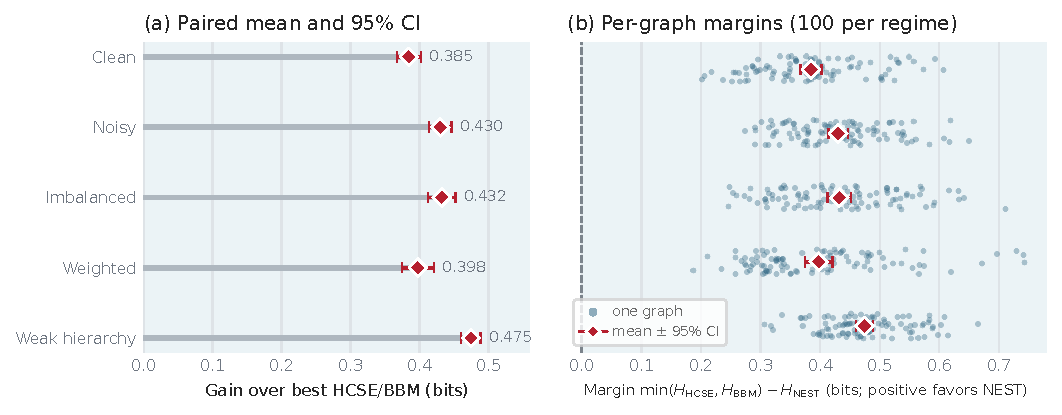
\includegraphics[width=\textwidth]{figures/benchmark_entropy.pdf}
  \caption{Paired advantage over external structural-entropy methods. For graph
  $g$, the margin is
  $M_g=\min(H^T_{\mathrm{HCSE},g},H^T_{\mathrm{BBM},g})-H^T_{\mathrm{NEST},g}$,
  so positive values favor \NEST. (a) Regime mean and paired 95\% confidence
  interval. (b) Each blue dot is one of 100 sealed graphs per regime; vertical
  jitter only separates overlapping dots. Red diamonds are regime means and
  horizontal whiskers are their 95\% confidence intervals. All 500 margins are
  positive.}
  \label{fig:entropy}
\end{figure}

\emph{Lower entropy coincides with better planted-hierarchy recovery on
average, but not on every graph} (Q3). Fine-level dendrogram purity is
\PurityFineNEST{} for \NEST, versus \PurityFineHCSE{} for HCSE and
\PurityFineBBM{} for oracle-$k$ BBM; the paired gains are
$\PurityFineGainHCSE\!\pm\!\PurityFineGainHCSECI$ and
$\PurityFineGainBBM\!\pm\!\PurityFineGainBBMCI$. Coarse-level gains are
$\PurityCoarseGainHCSE\!\pm\!\PurityCoarseGainHCSECI$ and
$\PurityCoarseGainBBM\!\pm\!\PurityCoarseGainBBMCI$. \NEST's fine purity is
nonetheless lower than HCSE's on \PurityFineLowerHCSE{} graphs, so entropy is
not a proxy for recovery on an individual instance.

\subsection{The operator audit}
\emph{Constructor quality and NNI-local optimality are different properties}
(Q1, Q2). Table~\ref{tab:operator} applies the same
two-stage refinement to each constructor's output: one-NNI descent commits the
best decreasing move until none remains, and the two-move escape then accepts
only a lower-entropy endpoint of a bounded pair. One-step NNI improves every
SE-agglomerative and oracle-BBM tree, and after that certificate the two-move
escape still improves 62\% and 93\% of them. On \BBMBudgetHits{} BBM trees
descent reached the $M=100$ move budget, so the BBM drops are lower bounds. Paris trees are improved in 74\%
and then 41\% of graphs. HCSE trees are nearly NNI-locally optimal, with rates
of 3\% and 4\%, yet their mean entropy exceeds that of Paris in every regime of
Table~\ref{tab:main-h}.

\begin{table}[t]
\centering\small
\caption{NNI refinement audit over 500 graphs. Drop is mean reduction relative
to raw $H^T$; improved is the fraction of graphs with a strict reduction.
Two-move values are additional to one-NNI descent, and time excludes initial
tree construction.}
\label{tab:operator}
\begin{tabular*}{\textwidth}{@{\extracolsep{\fill}}lccccc@{}}
\toprule
& \multicolumn{2}{c}{One-NNI descent}
& \multicolumn{2}{c}{Two-move escape}
& \shortstack{Refinement\\time} \\
\cmidrule(lr){2-3}\cmidrule(lr){4-5}
Constructor
& \shortstack{Entropy\\drop}
& \shortstack{Graphs\\improved}
& \shortstack{Extra entropy\\drop}
& \shortstack{Graphs further\\improved}
& (s) \\
\midrule
SE--agglomerative & 1.97\% & 100\% & 0.14\% & 62\% & 0.642 \\
Paris & 0.07\% & 74\% & 0.06\% & 41\% & 0.388 \\
HCSE & 0.00\% & 3\% & 0.00\% & 4\% & 0.108 \\
BBM$^\dagger$ & 14.02\% & 100\% & 0.46\% & 93\% & 1.962 \\
\bottomrule
\end{tabular*}
\end{table}




\subsection{Components and exact optimality}
\emph{Every component of {\upshape\NEST} contributes.} On a separate frozen 50-graph
subset (full ablation table in \ablationdetails), starting from SE agglomeration, the
candidate pool improves 34 graphs, one-NNI descent then improves 45, and the
two-move escape adds gains on 30. The main benchmark's verifier checks hashes,
schema, paired seeds, unique keys, and monotonicity of committed NNI endpoints
across its 3,500 method records and 500 generator manifests.


\emph{On exactly solvable graphs, 32 coalescent starts reach the global optimum
in \ScaleCombinedExact{} cases} (Q4). Disjoint calibration fixed $q=32$; we
then sealed 250 graphs at $n=12$, 100 at $n=14$, and 25 at $n=16$ across the
same five regimes. Every method receives exactly 32 candidates: coalescent
starts for \NEST; eight seeded HCSE calls at each target height 2--5; and
label-free BBM calls cycling through $k=2,\dots,8$ (four or five per $k$). The
deterministic \NEST pool is excluded from this budget. HCSE is nearly
deterministic, returning at most \HCSEMaxDistinct{} distinct entropies per
graph, whereas BBM returns \BBMDistinctRange{}. Selection uses only structural entropy, and the
exact dynamic program is consulted afterward. Table~\ref{tab:exact-scale}
reports 2/375 exact hits for HCSE and 1/375 for label-free BBM, with exact
binomial intervals for \NEST at each size. The interval widens to
[68.78, 97.45]\% at $n=16$, where only 25 graphs were audited. Every block has
status zero, matching SHA-256 seals, complete seed coverage, and independently
recomputed summaries; a fresh rerun of 15 of these graphs reproduced every
$H^*$ and every \NEST outcome.

\begin{table}[t]
\centering\small
\caption{Sealed exact-optimum audit on independently generated HSBMs with $n$
vertices and 32 candidates per method: coalescent starts for \NEST, target
heights for HCSE, and label-free cluster counts for BBM. Exact columns report
optimum hits over the listed graphs. The \NEST interval is an exact 95\% Clopper--Pearson
interval for its hit rate. Its relative gap is
$100(H^T_{\mathrm{NEST}}-H^*)/H^*$, reported as mean/worst; zero is optimal.
Candidate selection does not use $H^*$.}
\label{tab:exact-scale}
\begin{tabular*}{\textwidth}{@{\extracolsep{\fill}}rrccccc@{}}
\toprule
& & \multicolumn{3}{c}{Exact optima found}
& \multicolumn{2}{c}{\NEST diagnostics} \\
\cmidrule(lr){3-5}\cmidrule(lr){6-7}
$n$ & Graphs & \NEST & HCSE & BBM
& \shortstack{95\% hit-rate\\interval}
& \shortstack{Mean / worst\\relative gap} \\
\midrule
12 & 250 & \textbf{249/250} & 2/250 & 1/250 & [97.79, 99.99]\% & 0.00032\% / 0.07990\% \\
14 & 100 & \textbf{99/100} & 0/100 & 0/100 & [94.55, 99.97]\% & 0.00121\% / 0.12060\% \\
16 & 25 & \textbf{22/25} & 0/25 & 0/25 & [68.78, 97.45]\% & 0.03990\% / 0.44934\% \\
\bottomrule
\end{tabular*}
\end{table}


\subsection{Real networks}
\emph{{\upshape\NEST} also attains the lowest entropy on \RealWins{} real networks}
(Table~\ref{tab:real}). These networks lack a unique ground-truth hierarchy,
so this experiment measures objective minimization only. Paris is the closest
competitor, 0.004--0.019 bits behind.

\begin{table}[t]
\centering\small
\caption{Tree structural entropy $H^T$ (bits; lower is better) on four real
networks: Zachary karate club, Florentine families, Les Mis\'erables, and
Davis Southern women. Bold marks the lowest value per network.
BBM$^\dagger$ uses ground-truth $k$ for Karate and Louvain's $k$ otherwise.}
\label{tab:real}
\begin{tabular*}{0.90\textwidth}{@{\extracolsep{\fill}}lrrrr@{}}
\toprule
Method & Karate & Florent. & Les Mis. & Davis \\
\midrule
SE--agglomerative & 2.698 & 1.923 & 3.078 & 3.055 \\
Louvain--2L & 3.405 & 2.452 & 3.923 & 3.813 \\
Paris & 2.597 & 1.923 & 2.920 & 2.981 \\
HCSE & 2.929 & 2.172 & 3.930 & 3.206 \\
BBM$^\dagger$ & 3.330 & 2.254 & 3.199 & 3.387 \\
\midrule
\NEST\ (ours) & \textbf{2.586} & \textbf{1.919} & \textbf{2.916} & \textbf{2.962} \\
\bottomrule
\end{tabular*}
\end{table}


\section{Related Work}
\paragraph{Structural entropy and hierarchy construction.}
Li and Pan introduced structural information as an encoding-tree measure of
network organization \cite{li2016}. HCSE and BBM develop hierarchy
construction and balancing operations for this objective \cite{pan2025}.
SuperTAD proves binary sufficiency and uses it in contiguity-constrained dynamic
programs \cite{zhang2021supertad}; HCSE also notes the property \cite{pan2025}.
Our exact audit instead optimizes arbitrary vertex subsets.
The structural-entropy survey organizes the broader theory, optimization, and
application literature \cite{su2025survey}.
\NEST asks whether a returned tree is locally optimal under an exact topology
rotation and uses the answer as both a diagnostic and an optimizer.

\paragraph{Graph hierarchical clustering.}
Paris supplies an inexpensive agglomerative graph hierarchy related to
modularity \cite{bonald2018paris}. Louvain optimizes modularity
\cite{blondel2008}; we score its final partition as a two-level tree.
Dasgupta's cost and its revenue dual have inspired hierarchical algorithms with
guarantees \cite{dasgupta2016,moseley2017}. Because these objectives differ
from structural entropy, optimizing Eq.~\eqref{eq:tree-se} requires its own
local identity.

\paragraph{Exact inference and heuristic accuracy.}
Cluster trellises support exact hierarchical inference \cite{macaluso2021}.
Our routine is an SE specialization:
the prior binary-sufficiency property justifies the subset recurrence, while
our arbitrary-subset formulation differs from SuperTAD's contiguity-constrained
dynamic programs.

\paragraph{Local search in tree space.}
NNI is a classical neighborhood for evolutionary, or phylogenetic, trees; its
reconfiguration distance is itself nontrivial \cite{litrompzhang1996}. Recent
work studies NNI local search for hierarchical-clustering costs
\cite{jowhari2024}. PERCH uses purity-enhancing rotations during online tree
construction, while GRINCH combines rotations with longer-range grafts for
general linkage functions \cite{kobren2017perch,monath2019grinch}. Our formula
instead targets weighted graph structural entropy and exposes the two
cross-module weights controlling an NNI rotation, and evaluates the complete
objective on arbitrary weighted graphs.

\section{Limitations and Conclusion}
NNI is a local operator, and its certificate is not one of global optimality.
The two-move escape explores a bounded neighborhood, and multiway regions must
be resolved by a constructor before binary rotations can act on them. Lower
entropy raised planted purity on average but not on every graph, and no
coalescent restart recovered the strict planted tree in the exact and sampled
basin audits at $n=5$--$8$ and $n=12$. The exact solver is exponential, so the
near-optimality measurements cover only the declared 12--16-vertex suites.

We introduced \NEST, which uses an exact weighted NNI identity for monotone
refinement, a local-optimality certificate, and bounded escape from shallow
traps. It had the lowest entropy on all 500 paired graphs and reached the
exact optimum on \ScaleCombinedExact{} sealed instances at $n=12,14,16$,
versus 2/375 for HCSE and 1/375 for label-free BBM; this does not imply
global optimality beyond the audited suites.

\paragraph{Code and data availability.}
The implementation, sealed per-graph records, verifiers, and table generators
are available at \url{https://github.com/SuuTTT/nest-tamc-2026}.


\begin{credits}
\subsubsection{\ackname} This work was supported by the National Natural
Science Foundation of China (62576021).
\end{credits}

\bibliographystyle{splncs04}
\bibliography{refs}
\ifdefined\withappendix
\appendix
\section{Proof Details and Additional Basin Analysis}\label{app:proofs}

This appendix supplies proofs omitted from the 12-page main paper, the
component ablation, and additional finite-instance evidence; none of its claims
is needed to interpret the main experimental tables.

\paragraph{Proof of Theorem~\ref{thm:delta}.}
First suppose the three child modules have positive volume; the zero-volume
case follows by deleting modules with no incident positive-weight edge and
taking the zero-contribution limit. Only the terms for $A,B,C,X$, and $Y$ can
change. Omitting the common factor $1/\vol(V)$, their old and new contributions
are
\begin{align*}
 L_{\rm old}={}&g_A\log_2\frac{V_X}{V_A}
 +g_B\log_2\frac{V_X}{V_B}
 +g_X\log_2\frac{V_P}{V_X}
 +g_C\log_2\frac{V_P}{V_C},\\
 L_{\rm new}={}&g_A\log_2\frac{V_P}{V_A}
 +g_B\log_2\frac{V_Y}{V_B}
 +g_C\log_2\frac{V_Y}{V_C}
 +g_Y\log_2\frac{V_P}{V_Y}.
\end{align*}
Using $g_X=g_A+g_B-2W(A,B)$ and
$g_Y=g_B+g_C-2W(B,C)$, the coefficients of $g_A,g_B,g_C$ telescope to zero.
The remaining terms are
\[
 2W(A,B)\log_2(V_P/V_X)+2W(B,C)\log_2(V_Y/V_P).
\]
Restoring $1/\vol(V)$ proves Eq.~\eqref{eq:nni-delta}. External boundary
weights and $W(A,C)$ do not enter the delta.

\paragraph{Proof of Proposition~\ref{prop:atomic}.}
Delete $X$'s codeword and substitute $g_X=g_A+g_B-2W(A,B)$ in
Eq.~\eqref{eq:tree-se}; this gives Eq.~\eqref{eq:compress}. The symmetric
calculation for inserting $Y$ gives Eq.~\eqref{eq:merge}.

\paragraph{Proof of Proposition~\ref{prop:local}.}
Only moves with $\Delta\HT<-\varepsilon$ are committed, and their endpoint is
independently verified, so the objective never increases. The loop exits only
when the best enumerated move has $\Delta\HT\ge-\varepsilon$ or after $M$
moves; in the first case every legal move on an eligible binary parent--child
edge has $\Delta\HT\ge-\varepsilon$.

\paragraph{Proof of Proposition~\ref{prop:compound}.}
A pair is committed only after its final tree is fully recomputed and found to
have lower entropy than the tree preceding the pair. The first move is not
committed independently, so its sign cannot weaken the output guarantee. A
two-edge path may have a positive first delta and a negative net delta; the
regression witness in Sec.~\ref{sec:compound-search} instantiates this case.

\paragraph{Proof of Proposition~\ref{prop:binary} (included for completeness).}
At a node $P$, choose two children with disjoint leaf sets $A,B$, insert their
union $S=A\cup B$ below $P$, and make $A,B$ children of $S$. The objective
change is
\[
 -\frac{2W(A,B)}{\vol(V)}\log_2\frac{V_P}{V_S}\le 0.
\]
Repeated insertion converts every multiway node to binary without increasing
the objective.

\subsection{Exact and sampled basin probabilities}\label{app:basin}
The finite hit rates in the main paper do not supply a per-start probability.
For a fixed graph $G$, deterministic refinement map $F$, optimum $H^*$, and
start measure $\mu$, that probability is
\[
 p_G=\sum_T \mu(T)\,\mathbf{1}\{H^{F(T)}(G)=H^*(G)\}.
\]
It depends on the graph, start distribution, tie-breaking, and refinement
configuration.  The exact subset DP supplies $H^*$ but not $p_G$.

For $n\leq 8$ we enumerate all $(2n-3)!!$ unordered rooted binary labeled
topologies.  Uniform topology mass is not NEST's restart distribution. Under
the pairwise coalescent, a topology with child subtrees of $a,b$ leaves has
compatible-history count
\[
 h(T)=\binom{a+b-2}{a-1}h(T_A)h(T_B),\qquad
 \mu(T)=\frac{h(T)}{\prod_{k=2}^{n}\binom{k}{2}}.
\]
The history counts sum exactly to the denominator. Table~\ref{tab:basin-exact}
shows that the selected hard $n=8$ graph has exact coalescent basin mass
$p_G=0.252365$; because the standard pool misses it, 32 independent starts
give $1-(1-p_G)^{32}=0.999909$, not certainty.

\begin{table}[t]
\centering
\caption{Exact restart-basin probabilities for one fixed noisy HSBM at each
size. The All topologies column gives $(2n-3)!!$, the number of unordered
rooted binary labeled starting trees. Standard pool exact reports whether \NEST's
deterministic initializer pool reaches the global optimum $H^*$. $p_U$ is the
fraction of uniformly weighted starts refined to $H^*$; $p_C$ uses \NEST's
pairwise-coalescent restart distribution. Strict recovery requires every
planted fine and coarse block to appear as a clade.}
\label{tab:basin-exact}
\small
\begin{tabular*}{\textwidth}{@{\extracolsep{\fill}}rrcccc@{}}
\toprule
& & & \multicolumn{2}{c}{Optimum basin}
& \shortstack{Strict-recovery\\basin} \\
\cmidrule(lr){4-5}
$n$ & \shortstack{All\\topologies}
& \shortstack{Standard pool\\exact?}
& \shortstack{Uniform\\$p_U(H^*)$}
& \shortstack{Coalescent\\$p_C(H^*)$}
& \shortstack{Coalescent\\$p_C(\mathrm{strict})$} \\
\midrule
5 & 105     & yes & 100.000\% & 100.000\% & 0.000\% \\
6 & 945     & yes & 100.000\% & 100.000\% & 0.000\% \\
7 & 10,395  & yes & 100.000\% & 100.000\% & 0.000\% \\
8 & 135,135 & no  &  24.848\% &  25.237\% & 0.000\% \\
\bottomrule
\end{tabular*}
\end{table}


\subsection{Detailed 12-vertex method audit}
Table~\ref{tab:optimality} retains the full method and runtime breakdown for the
largest exact-audit stratum. The main paper reports the cross-size comparison.

\begin{table}[t]
\centering\scriptsize
\caption{Detailed budget-matched audit on 250 independently generated
12-vertex HSBMs. Candidates/graph is the number proposed before
structural-entropy-only selection; $H^*$ is revealed afterward. The successful
graphs column counts completed runs, whereas exact-optimum rates use all 250 graphs.
Relative gap is $100(H^T-H^*)/H^*$ (mean $\pm$ 95\% CI over successful
graphs), and zero is best. Time includes all candidates for one graph.}
\label{tab:optimality}
\begin{tabular*}{\textwidth}{@{\extracolsep{\fill}}lccccc@{}}
\toprule
Method
& \shortstack{Candidates\\per graph}
& \shortstack{Successful\\graphs}
& \shortstack{Exact optima\\count (rate)}
& \shortstack{Mean relative gap\\$\pm$ 95\% CI (\%)}
& \shortstack{Mean time\\per graph (s)} \\
\midrule
\NEST (coalescent) & 32 & 250/250 & \textbf{249 (99.6\%)} & \textbf{$0.000320\!\pm\!0.000629$} & 0.171 \\
HCSE & 32 & 250/250 & 2 (0.8\%) & $10.902\!\pm\!0.971$ & 0.024 \\
BBM (oracle $k$) & 32 & 248/250 & 1 (0.4\%) & $15.054\!\pm\!1.13$ & 0.402 \\
BBM (label-free) & 32 & 250/250 & 1 (0.4\%) & $10.237\!\pm\!0.593$ & 0.299 \\
SE agglomerative & 1 & 250/250 & 44 (17.6\%) & $1.764\!\pm\!0.268$ & $<0.001$ \\
\bottomrule
\end{tabular*}
\end{table}


At $n=12$, exact enumeration would require 13,749,310,575 topologies.
Table~\ref{tab:basin-mc} therefore uses direct Bernoulli sampling rather than
the earlier first-hit diagnostic. The estimates vary substantially by graph:
$8.07\%$--$46.43\%$ per start. On noisy-11 this implies only $93.23\%$ for 32
random starts (a conservative 95\% lower value of $91.87\%$), explaining why
the observed finite-suite success must not be read as a probabilistic
guarantee.

\begin{table}[t]
\centering
\caption{Restart success on eight hard $n=12$ graphs, using 10,000 independent
coalescent starts per graph. Graph IDs are regime--seed. $\hat p(H^*)$ is the
fraction of starts refined to the exact optimum; intervals are exact 95\%
Clopper--Pearson intervals. $q_{32}=1-(1-\hat p)^{32}$ estimates the chance
that at least one of 32 independent starts succeeds; lower $q_{32}$ substitutes
the lower confidence limit for $\hat p$. Strict planted recovery occurred
0/10,000 times on every graph (per-graph 95\% upper bound $0.0369\%$).}
\label{tab:basin-mc}
\small
\begin{tabular*}{\textwidth}{@{\extracolsep{\fill}}lcccc@{}}
\toprule
Graph
& \shortstack{Successful starts\\$\hat p(H^*)$}
& \shortstack{95\% interval\\for $\hat p$}
& \shortstack{Predicted 32-start\\success $q_{32}$}
& \shortstack{Conservative\\lower $q_{32}$} \\
\midrule
noisy-0  & 17.19\% & [16.46, 17.94]\% & 99.761\% & 99.683\% \\
noisy-8  & 14.61\% & [13.92, 15.32]\% & 99.362\% & 99.175\% \\
noisy-9  & 20.56\% & [19.77, 21.37]\% & 99.937\% & 99.913\% \\
imbal.-0 & 46.43\% & [45.45, 47.41]\% & 100.000\% & 100.000\% \\
weak-9   & 30.61\% & [29.71, 31.52]\% & 99.999\% & 99.999\% \\
noisy-11 &  8.07\% & [ 7.54,  8.62]\% & 93.229\% & 91.872\% \\
noisy-17 & 17.75\% & [17.01, 18.51]\% & 99.808\% & 99.743\% \\
weak-17  & 17.86\% & [17.11, 18.63]\% & 99.816\% & 99.754\% \\
\bottomrule
\end{tabular*}
\end{table}


Objective success is deliberately separated from strict planted recovery.
No one of the 80,000 hard-case endpoints contained every planted fine and
coarse block as a clade; the exact $n=8$ enumeration likewise gives zero mass.
This strict event is stronger than dendrogram purity and exposes objective--
recovery misalignment on these small realized HSBMs. Thus the restart evidence
supports optimization of $H^T$, not a claim that every entropy optimum equals
the generator's planted hierarchy.

\paragraph{Component ablation.}
Table~\ref{tab:ablation} gives the cumulative ablation summarized in
Section~\ref{sec:experiments}.

\begin{table}[t]
\centering\small
\caption{Cumulative \NEST ablation on 50 paired HSBMs (10 per regime). Each $+$ row adds one
component to the preceding row. The candidate pool selects the lowest-entropy
initial tree among SE agglomeration, recursive SE, and Paris.
$\Delta H^T=H^T_{\mathrm{previous}}-H^T_{\mathrm{row}}$, so positive values are
improvements; the final column counts graphs with a strict decrease.}
\label{tab:ablation}
\begin{tabular*}{0.88\textwidth}{@{\extracolsep{\fill}}lccc@{}}
\toprule
Variant
& \shortstack{Mean $H^T$\\(bits)}
& \shortstack{Mean $\Delta H^T$\\(bits)}
& \shortstack{Graphs\\improved} \\
\midrule
SE agglomeration & 3.1435 & -- & -- \\
+ candidate pool & 3.1041 & 0.0394 & 34/50 \\
+ one-NNI descent & 3.0794 & 0.0247 & 45/50 \\
+ two-move escape & 3.0759 & 0.0035 & 30/50 \\
\bottomrule
\end{tabular*}
\end{table}


\paragraph{Refinement runtime.}
Figure~\ref{fig:runtime} complements Table~\ref{tab:operator} with the
quality--time trade-off of each initializer.

\begin{figure}[h]
  \centering
  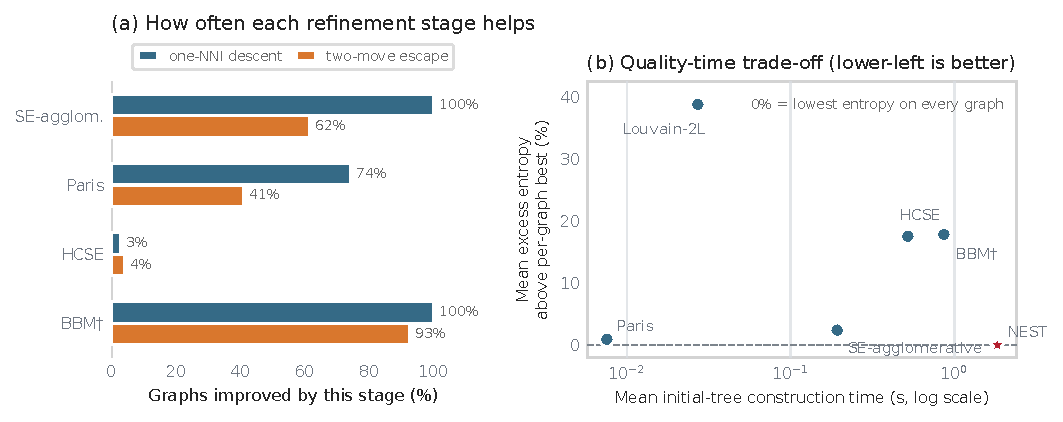
\includegraphics[width=0.94\textwidth]{figures/operator_runtime.pdf}
  \caption{NNI refinement over 500 graphs. (a) Blue is the fraction of initial
  trees improved by repeated best-decreasing NNI moves. After no single move
  helps, the two-move escape may cross one uphill intermediate tree; orange is
  the fraction whose final endpoint improves further. (b) Each point is an
  initializer. Excess entropy is
  $100(H^T-H^T_{\mathrm{best}})/H^T_{\mathrm{best}}$, where
  $H^T_{\mathrm{best}}$ is the lowest value on the same graph; thus zero is
  best. The horizontal axis is mean construction time in log seconds, so
  lower-left is better. Times include Python allocation tracing.}
  \label{fig:runtime}
\end{figure}

\paragraph{A graph-only lower bound.}
For an additional graph-only certificate, an edge-LCA expansion gives
\begin{equation}
H^T(G)=\sum_{uv\in E}\frac{w_{uv}}{\vol(V)}
\log_2\frac{V_{\operatorname{lca}(u,v)}^2}{d_ud_v}
\ge \sum_{uv\in E}\frac{w_{uv}}{\vol(V)}
\log_2\frac{(d_u+d_v)^2}{d_ud_v}.
\label{eq:edge-bound}
\end{equation}
The inequality follows from
$V_{\operatorname{lca}(u,v)}\ge d_u+d_v$. It is a universal lower bound, but
the exact dynamic program gives the sharper certificates reported below.

\fi
\end{document}
